\chapter[Introduction Générale]{Introduction Générale}
\label{Introduction}

\chapterabstract
{
Dans ce chapitre introductif, nous allons présenter d'une part l'organisme d'accueil « Direction de la Météorologie 
Nationale » où le stage a été effectué, ses stratégies, ses missions et ses domaines d'activité. D'autre part, 
nous présenterons aussi les enjeux liés à la prévision de la visibilité, ainsi que l’état des lieux en ce qui concerne 
l'estimation de la visibilité grâce au Datamining à partir de diverses sources de données en utilisant divers algorithmes dans différentes plateformes.
Les objectifs du stage et la stratégie suivie pour les atteindre seront explicités en fin de ce chapitre.
}
\pagestyle{plain}

%%%%%%%%%%%%%%%%%%%%%%%%%%%%%%%%%%%%%%%%%%%%%%%%%%%%%%%%%%%%%%%%%%%%%%%
\section{Organisme d’accueil: Direction de la Météorologie Marocaine}
%%%%%%%%%%%%%%%%%%%%%%%%%%%%%%%%%%%%%%%%%%%%%%%%%%%%%%%%%%%%%%%%%%%%%%%
\begin{wrapfigure}{l}{0.2\textwidth}
    \vspace{-0.5 cm}    
    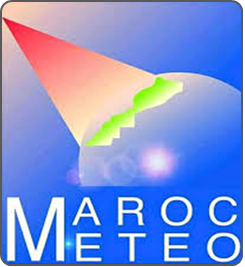
\includegraphics[width=0.2\textwidth]{img/logo_dmn.png}
    \vspace{-1 cm}
\end{wrapfigure}
A travers la Direction de la Météorologie Nationale (DMN, souvent appelé Maroc Météo par les usagers), le Maroc dispose d’un outil à même d'assurer et de coordonner l'ensemble des activités météorologiques et climatiques. La DMN, en tant que service public, a pour objectif central de promouvoir une assistance technique et scientifique dans les sciences de l'atmosphère. Sa mission est de servir les intérêts socio-économiques de la nation et de contribuer à la
sauvegarde des vies et des biens de la population, à travers son métier qui consiste en (Cf. Fig. \ref{fig:MissionDMN}) :
\begin{itemize}
\item[\ding{224}] l'observation et la mesure météorologiques,
\item[\ding{224}] la prévision,
\item[\ding{224}] la veille et le suivi du climat,
\item[\ding{224}] l'assistance météorologique aux secteurs économiques : la navigation aérienne, les activités marines, l'agro-météorologie, l'hydro-météorologie et l'environnement, etc.\\
\end{itemize}

\begin{figure}[!h]
\centering
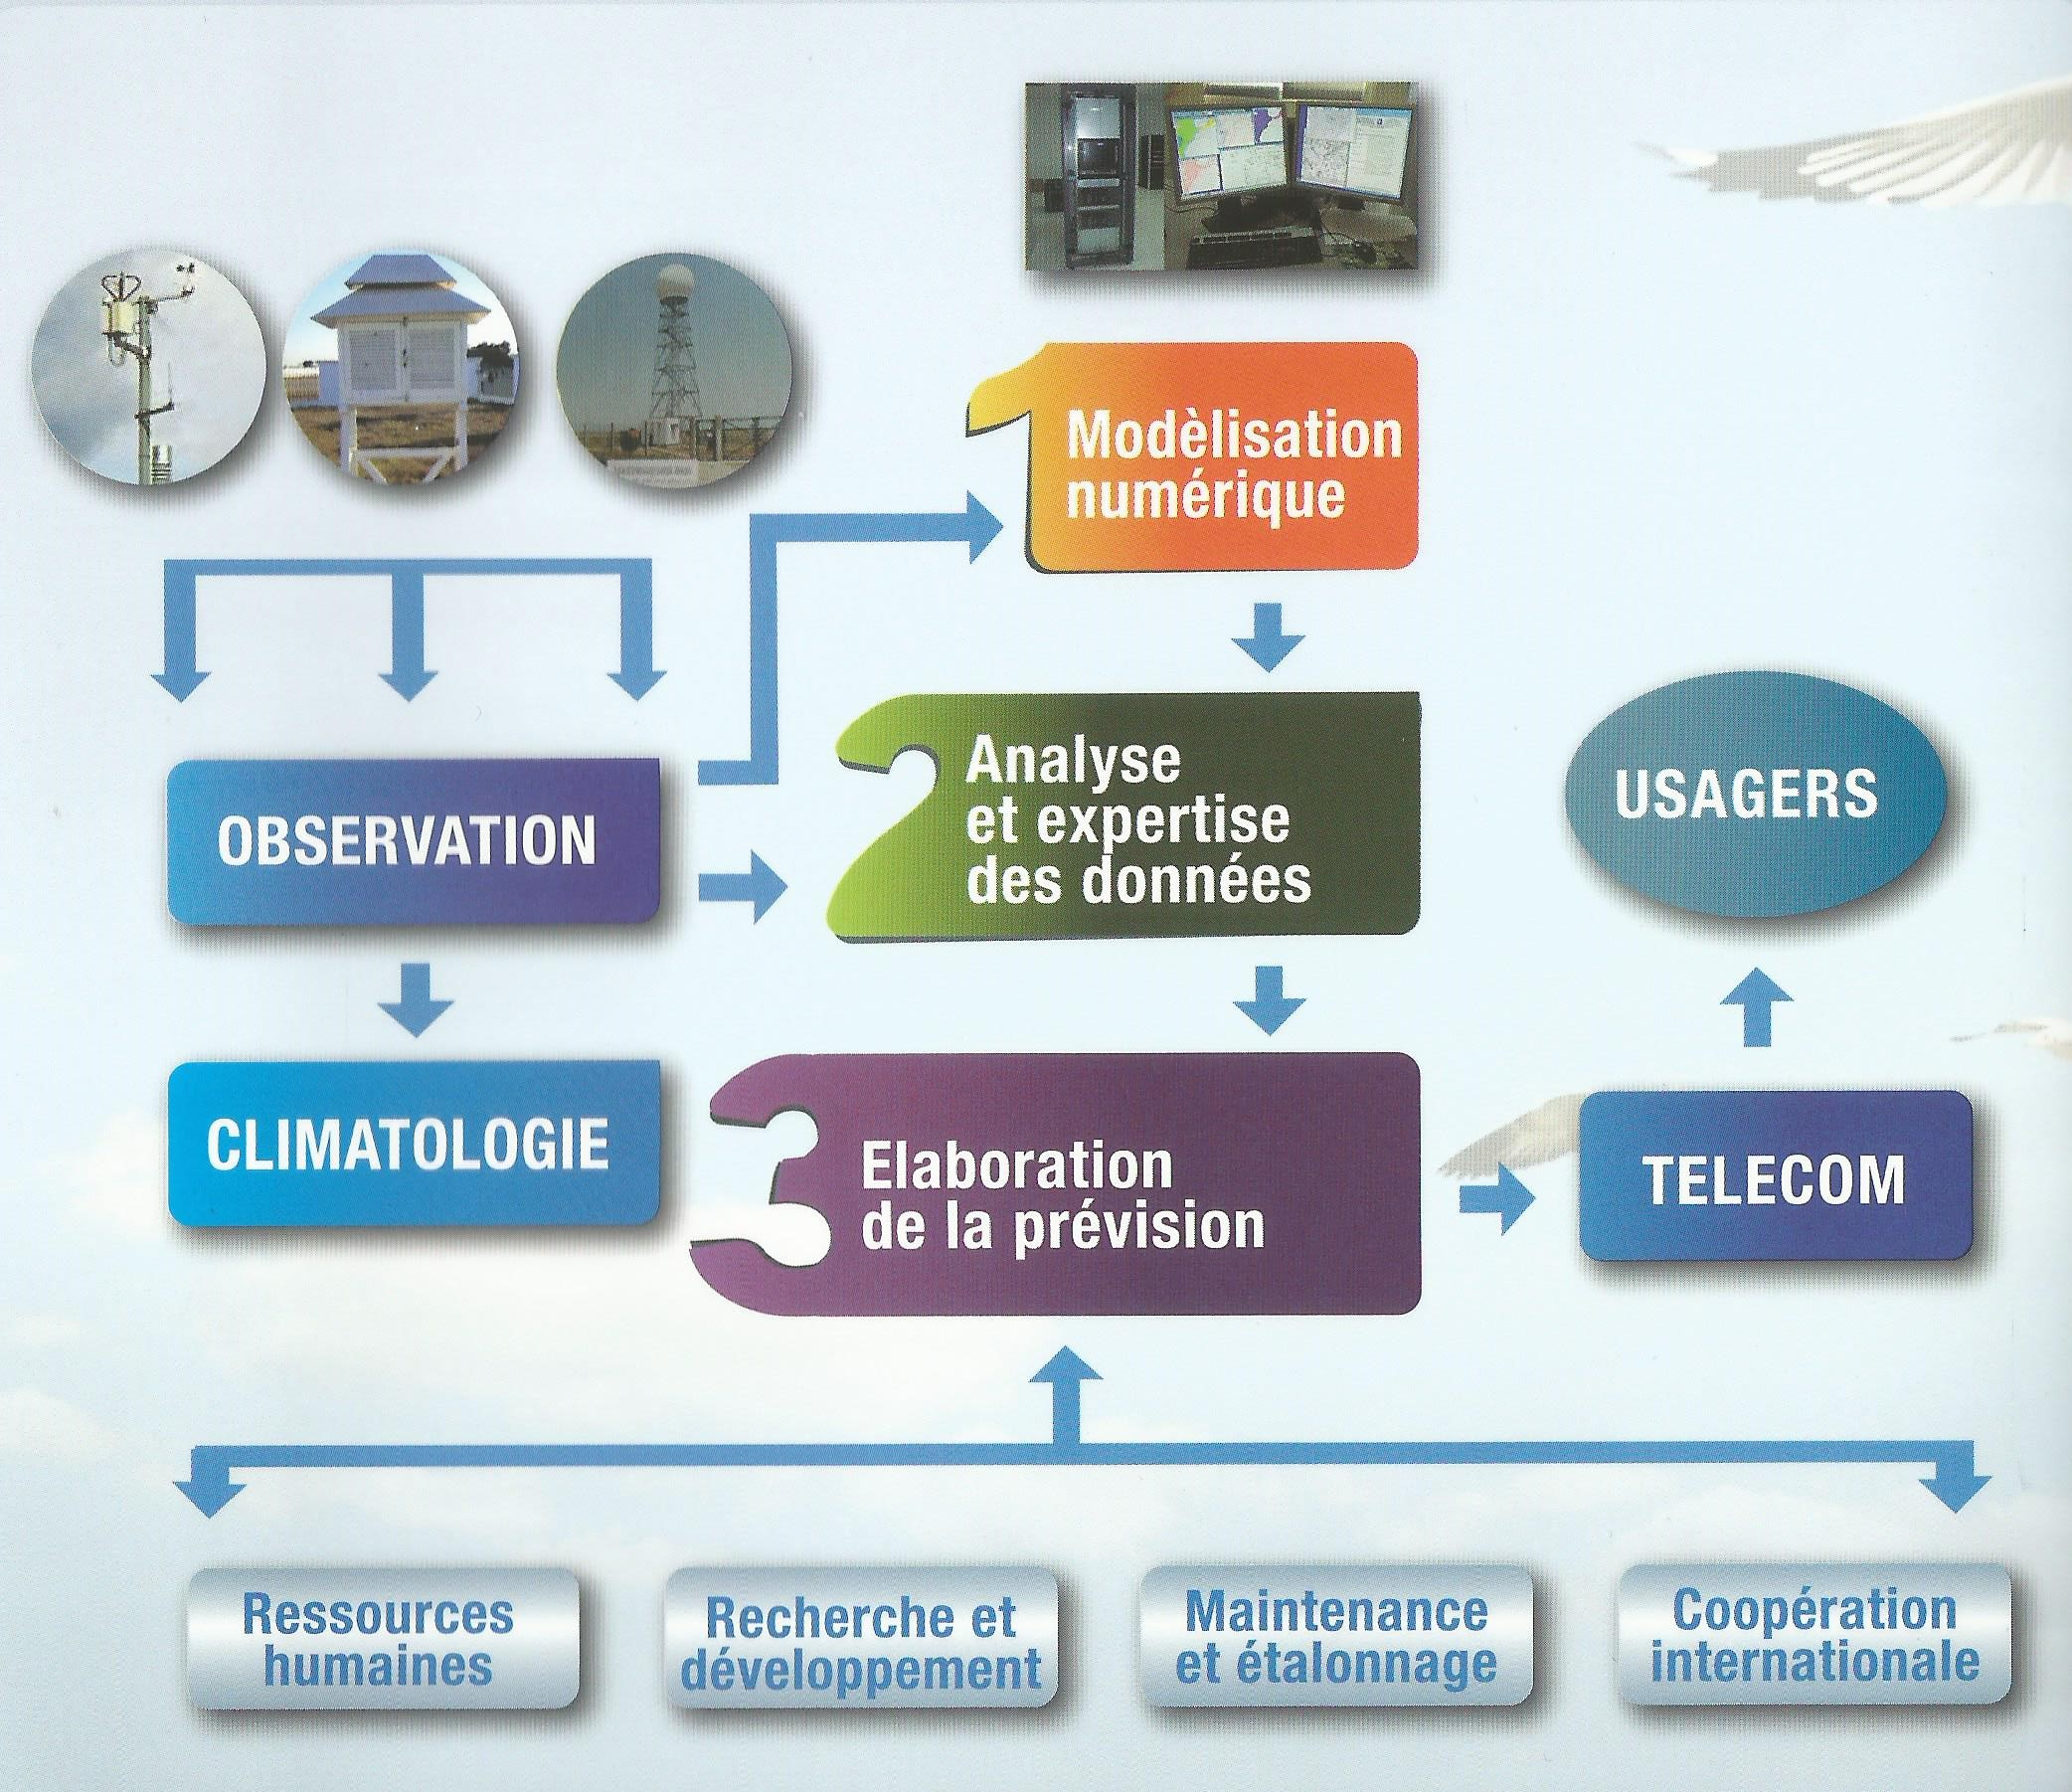
\includegraphics[width=10 cm, height= 7 cm]{img/DMN.jpeg}
\caption{Représentation schématique des principales activités de Maroc Météo}
\label{fig:MissionDMN}
\end{figure}

Les missions de la DMN décrites dans le décret No. 2-94-724 du 21 Novembre 1994 sont :
\begin{itemize}
\item[\ding{224}] Assurer les activités relatives aux
informations météorologiques et
climatologiques nécessaires pour satisfaire tous les besoins des usagers au plan national et assurer les échanges internationaux de données en application des
accords ratifiés par le Royaume du Maroc.
\item[\ding{224}] Effectuer des études et recherches atmosphériques, de météorologie et de
climatologie théoriques, expérimentales et appliquées ainsi que les études et les recherches connexes en rapport avec sa mission.
\item[\ding{224}] Participer à la préparation des accords internationaux en liaison avec les administrations intéressées concernant les domaines de sa compétence et
d’établir les textes réglementaires relatifs à la météorologie et en assurer l’exécution.\\
\end{itemize}
 
 Pour répondre à sa mission, Maroc Météo dispose de ressources humaines hautement qualifiées dans les domaines de la météorologie, de l'informatique, des réseaux et télécommunications et de la maintenance. Ainsi, la DMN dispose actuellement de 746 fonctionnaires (Cf. Tab. \ref{tab:effectifDMN}) dont 31.9\% de cadres, 58.4\% de techniciens et 9.7\% d’adjoints techniques. Il est à noter que le personnel aux niveaux des régions et des Centres Provinciaux Météorologiques (CPM, antérieurement appelé « station ») représente 56\%.\\

\begin{table}[!h]
\centering
\begin{tabular}{lrrr}
\hline
Corps & Homme & Femme & Total \\
\hline
Cadre & 167 (70.2\%) & 71 (29.8\%) & 238 (31.9\%) \\
Technicien & 303 (69.5\%) & 133 (30.5\%) & 436 (58.4\%) \\
Agent & 48 (66.7\%) & 24 (33.3\%) & 72 (9.7\%) \\
\hline
Total & 518 (69.4\%) & 228 (30.6\%) & 746 (100\%) \\
\hline
\end{tabular}
\caption{Répartition de l'effectif actuel (jusqu'à juillet 2017) à Maroc Météo par corps et par genre}
\label{tab:effectifDMN}
\end{table}
Elle dispose aussi d'un ensemble de moyens techniques performants:

\begin{enumerate}
\item Des moyens d'observation:
    \begin{itemize}
    \item[\ding{224}] Un réseau d'observation des phénomènes météorologiques diversifié:
        \begin{itemize}
        \item[\ding{74}] Observation au sol : un réseau classique et automatique de mesure de paramètres météorologiques
        \item[\ding{74}] Observation en altitude : un réseau de 7 radars, un réseau foudre facilitant la localisation des cellules orageuses, des imageries Satellitaires, un radio-sondage.
        \item[\ding{74}] Réseau de mesure de la qualité de l'air
        \end{itemize}
    \item[\ding{224}] Un laboratoire de métrologie
    \end{itemize}
\item Des moyens de prévision :
    \begin{itemize}
     \item[\ding{224}] Des modèles numériques de prévision du temps:
     \begin{itemize}
        \item[\ding{74}] Les modèles de prévision du temps sur des échelles spatiales et temporelles différentes: Albachir (7.5km sur le Maroc pour 72 heures de prévision), NORAF (18km sur le nord de l'Afrique pour 72 heures de prévision), AROME (2.5km sur le Maroc pour 48 heures de prévision) et COBEL-ISBA (modèle colonne pour la prévision du brouillard à l'aéroport Nouasseur, et qui donne des prévisions pour 12 heures)
        \item[\ding{74}] Modèle SWAN : c'est un modèle d'eaux peu profondes «Shallow water» de troisième génération permettant l’estimation des paramètres des vagues dans les zones côtières, les lacs et les estuaires à partir des conditions atmosphériques (forçage du vent) et du fond marin.
        \item[\ding{74}] Modèle WAVEWATCH III version 2.22 pour la prévision de l’état de la mer
        \item[\ding{74}] Modèle MOTHY utilisé principalement pour prédire la dérive de polluants ou d'objets flottants sur la surface de l'océan.
        \item[\ding{74}] ARPEGE-Climat et ALADIN-Climat: deux modèles opérationnels utilisés pour la prévision saisonnière et la recherche sur le climat.
     \end{itemize}
     \item[\ding{224}] Des modèles de prévision de la qualité de l'air : MOCAGE et PERLE
     \item[\ding{224}] Synergie: système d'intégration et de visualisation des données météorologiques
    \end{itemize}    
\item Des moyens de calcul de plus en plus performants : Maroc Météo dispose d'un calculateur HPC d'IBM qui est une machine parallèle destinée pour le calcul intensif et composée de 114 lames de calcul, 2 lames de compilation et de développement. Ces nœuds sont interconnectés via un réseau très rapide InfiniBand. Le système a une capacité totale théorique de calcul allant jusqu’à 8.3 Téra Flops, une mémoire centrale de 1.95 TB et une mémoire de masse d’environ 52 TB.
\item Des moyens de transmission de données : Serveux Fax, Serveur FTP, Transmet, Messir com, Extranet, etc.
\item Des moyens de télécommunications :  Liaisons spécialisées, VPN, Internet.
\item Domiciliation du système GISC (Global Information System Centre -WIS terminology-) au Maroc (seul pays africain avec l’Afrique du Sud) dans le système d’information de l’organisation mondiale de la météorologie OMM. Ce nouveau système d’information international destiné à faciliter et développer l’échange de données météorologiques, climatiques et hydrologiques et
à réduire les dépenses correspondantes.\\
\end{enumerate}

Maroc Météo assure à ses usagers une veille météorologique continue 24H sur 24 et 7J sur 7, sur l'ensemble du pays. Elle offre à ses partenaires:

\begin{itemize}
\item[\ding{74}] Un ensemble de bulletins de prévisions météorologiques réguliers
\item[\ding{74}] Des bulletins d'alerte aux différents secteurs soci-économiques
\item[\ding{74}] Des images radar et satellites permettant la localisation, et le suivi des cellules orageuses
\item[\ding{74}] Des données et études climatologiques sur tout le Royaume
\item[\ding{74}] Une observation et surveillance des impacts foudre
\item[\ding{74}] Une surveillance de l'état de la qualité de l'air au Maroc.\\
\end{itemize}

Dans le but d'accroître ses performances, Maroc Météo a mis en place une stratégie lui permettant d'améliorer en continue ses prestations. La DMN est certifié ISO 9001-2008 par « Bureau Véritas Certification ». En tant que prestataire de service à la navigation aérienne, la DMN est également certifié conforme aux exigences de l’OACI. Dans le cadre de cette politique qualité, Maroc Météo s'engage :
\begin{enumerate}
\item à ce que ses prestations soient réalisées conformément au Système de Management de la Qualité;
\item à déployer les ressources nécessaires pour répondre aux exigences de ses clients et usagers;
\item à engager une Écoute Client attentive aux besoins spécifiques de ses différents partenaires et usagers, afin de mieux répondre à leurs attentes;
\item à respecter les exigences réglementaires et légales;
\item à mobiliser l'ensemble de son personnel autour de sa politiques qualité;
\item à s'assurer que l'application de cette politique demeure pertinente, adéquate et efficace.\\
\end{enumerate}

Quelques chiffres clé de Maroc Météo peuvent être récapitulés comme suit :
\begin{itemize}
\item[\ding{224}] Plus de 450 bulletins météorologiques par jour
\item[\ding{224}] Des capacités de calcul dépassant les 8300 milliards d'opérations par seconde
\item[\ding{224}] Un réseau d'observation important : 43 stations météorologiques principales
\item[\ding{224}] Un réseau climatologique composé de 528 postes dont 432 pluviomètres
\item[\ding{224}] 156 stations automatiques météorologiques au niveau des zones difficiles d'accès
\item[\ding{224}] 5 stations maritimes aux ports de : Tanger, Mohammedia, Casablanca, Jorf-Lasfar et Essaouira
\item[\ding{224}] un réseau radar de 7 stations situées à Nouasseur, Agadir, Fès, Khouribga, Larache, Bengrir et Debdou
\item[\ding{224}] une réseau foudre constitué de 4 capteurs situés à Casablanca, Fès, Ouarzazate, Agadir et oujda
\item[\ding{224}] 29 stations fixes de mesure de la qualité de l'air et deux laboratoires mobiles
\item[\ding{224}] Le taux de réussite des services météorologiques dépasse les 90\% pour les prévisions à 2
 heures
 \item[\ding{224}] Des ressources humaines hautement qualifiées avec un taux d'encadrement dépassant 26\%.\\
\end{itemize}

A compter de 2015, la DMN dispose d’un nouvel organigramme en tant que Service d’Etat Géré d’une Manière Autonome (SEGMA) sous la tutelle du Ministère de l'Équipement, du Transport, de la Logistique et de l'Eau. Ainsi, la DMN se compose des 5 divisions, 3 centres et 6 directions régionales :
\begin{itemize}
\item[\ding{224}]  Division des Affaires Administratives et de la Formation (DAAF)
\item[\ding{224}]  Division du Budget et de la Gestion Financière (DBGF)
\item[\ding{224}]  Division des Affaires Techniques et de l’Équipement (DATE)
\item[\ding{224}]  Division de la Communication et de la Commercialisation (DCC)
\item[\ding{224}]  Division du Développement, de la Coopération et de la Qualité (DDCQ)
\item[\ding{224}]  Centre National de Prévisions (CNP)
\item[\ding{224}]  Centre National de Recherches Météorologiques et des Systèmes d’Information
(CNRMSI)
\item[\ding{224}]  Centre National du Climat (CNC)
\item[\ding{224}]  Direction Régionale Météorologique du Centre
\item[\ding{224}]  Direction Régionale Météorologique du Centre-Est
\item[\ding{224}]  Direction Régionale Météorologique du Centre-Ouest
\item[\ding{224}]  Direction Régionale Météorologique du Nord-Est
\item[\ding{224}]  Direction Régionale Météorologique du Nord-Ouest
\item[\ding{224}]  Direction Régionale Météorologique du Sud\\
\end{itemize}
 
Chaque division, centre et direction régionale se compose de services. Parmi ces services celui de la \textbf{Modélisation Numérique} qui fait partie du CNRMSI, où j'ai effectué mon stage. Les activités stratégiques du service de Modélisation Numérique tournent autour de :
 \begin{itemize}
 \item[\ding{224}] L'amélioration de la qualité de la prévision par l'introduction et le contrôle du maximum d'observations locales et par la modélisation
 \item[\ding{224}] Le développement d'outils d'aide à la prévision notamment en matière de détection et de prévision du brouillard
 \item[\ding{224}] Le renforcement de notre présence dans la communauté scientifique par des études dans le domaine de la modélisation numérique et l'assimilation de données
 \end{itemize}



%%%%%%%%%%%%%%%%%%%%%%%%%%%%%%%%%%%%%%%%%%%%%%%%%%%%%%%%%%%%%%%%%%%%%%%
\section{Enjeux de la prévision de la visibilité}
%%%%%%%%%%%%%%%%%%%%%%%%%%%%%%%%%%%%%%%%%%%%%%%%%%%%%%%%%%%%%%%%%%%%%%%
Parmi les différents phénomènes météorologiques liés à la visibilité réduite et qui peuvent impacter la circulation aérienne, maritime et routière, le brouillard reste un de ceux qui perturbent souvent ces trois secteurs. En effet, la définition internationale du brouillard consiste en une suspension, au voisinage du sol, de poussières, de gouttelettes ou de particules glacées réduisant la visibilité horizontale à une valeur inférieure à 1 km \citep{def_broui}. Quand la visibilité est réduite à moins de 5 km tout en dépassant 1 km, le phénomène est appelé brume. Il est à noter que les nuisances du brouillard sur la vie socio-économique sont importantes. Ainsi, le brouillard peut entraîner des retards importants et des perturbations dans les systèmes de transport aérien, maritime et routier.\\

Pour le transport routier au Maroc, un épais brouillard était la principale cause de 6 accidents sur l’autoroute Casablanca-Mohammedia, le 17 janvier 2011, provoquant d’importants dégâts touchant une cinquantaine de véhicules et une dizaine de blessés. Un autre brouillard épais qui a été observé au cours de la nuit du 23 au 24 Décembre 2013, a causé un carambolage impliquant plusieurs véhicules, sur l’autoroute entre Casablanca et El Jadida (située à 90 km au sud de Casablanca). Cet événement de brouillard a fait 6 morts et 24 blessés (Cf. Fig. \ref{eco}).\\ \\ \\ \\ \\
\begin{figure}[!h]
\parbox{9cm}{ 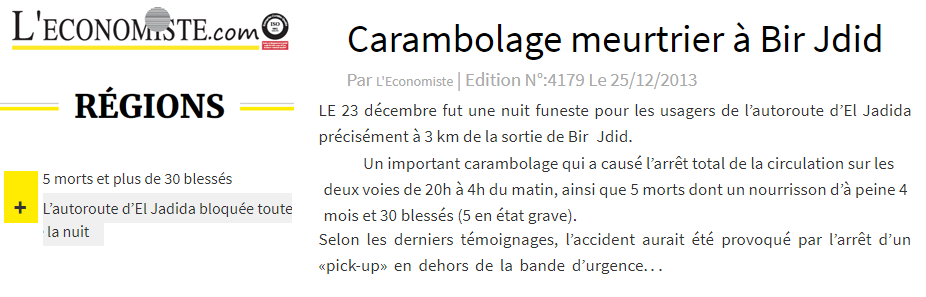
\includegraphics[width=8cm, height=3cm]{img/econ.png}
}
\parbox{5cm}{\caption{ Accident meurtrier sur l’autoroute entre Casablanca et El Jadida au cours de la nuit du 23-24 Décembre 2013 à cause d’un épais brouillard (Source : L’Economiste)}
\label{eco}
}
\end{figure}


Concernant la circulation aérienne, les vols vers un aéroport couvert de brouillard sont souvent reportés ou annulés, menant à des conséquences économiques directes et indirectes.  L’épais brouillard du 20 Janvier 2008 (Cf. Fig. \ref{aujour}) a engendré le
déroutement de 21 avions, devant atterrir à l’aéroport Mohammed V, vers les aéroports de Marrakech, Agadir, Tanger, Fès et Ouarzazate. 
Ainsi, le brouillard a perturbé encore une fois le trafic aérien du royaume le 05 avril 2015 (Cf. Fig. \ref{aujour}). Pour les compagnies aériennes, le déroutement
des avions est synonyme de dépenses plus importantes en kérosène, de prise en charge de passagers, de
remboursements, etc.\\
\begin{figure}[!h]
\parbox{9cm}{
\centering
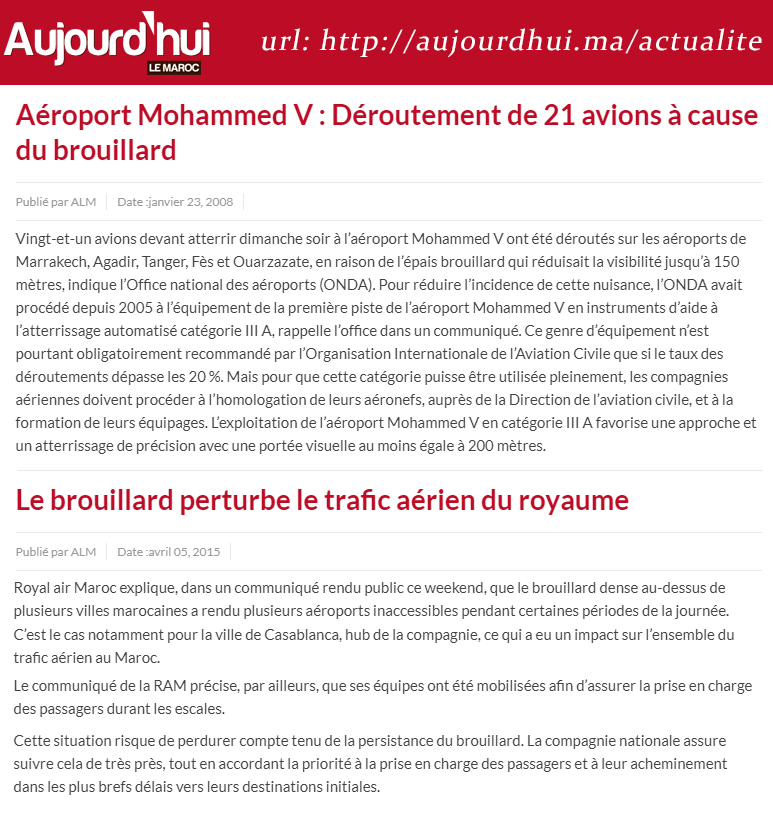
\includegraphics[width=8cm, height=8.2cm]{img/aujourd.png}
}
\parbox{5cm}{
\caption{ Exemples des perturbation d'aéroports du Royaume à cause du brouillard (Source: Aujourd’hui Le Maroc)}
\label{aujour}
}
\end{figure}

À travers ce qui précède, Il s'avère ainsi qu'une bonne prévision de la visibilité horizontale sera d'un grand apport pour les prévisionnistes météorologiques; ce qui réduira en conséquence les impacts néfastes sur certains secteurs socio-économiques et aidera ainsi à une bonne gestion des transports en condition de basse visibilité.


\newpage
%%%%%%%%%%%%%%%%%%%%%%%%%%%%%%%%%%%%%%%%%%%%%%%%%%%%%%%%%%%%%%%%%%%%%%%
\section{Platformes et algorithmes utilisés pour l'estimation de la visibilité : État des lieux}
%%%%%%%%%%%%%%%%%%%%%%%%%%%%%%%%%%%%%%%%%%%%%%%%%%%%%%%%%%%%%%%%%%%%%%%
Dans la littérature scientifique, plusieurs recherches ont abordé la problématique de la détection et la prévision des basses visibilités selon diverses approches (classification et régression) en utilisant diverses plateformes open-sources.
\cite{gultepe2007} ont indiqué, dans l’article de synthèse des travaux de recherche réalisés sur la
thématique du brouillard, que la prévision des événements de basses visibilités en particulier le
brouillard par les modèles de prévision numérique du temps reste difficile, car ce type de phénomène
météorologique dépend de plusieurs facteurs aux échelles locale et globale. Comme alternative, les
chercheurs se sont penchés sur une autre approche qui consiste à utiliser de nouvelles techniques et
méthodologies statistiques dans le but d’élaborer et de développer des modèles pour aider les prévisionnistes à améliorer la prédiction des événements à visibilité réduite dans les aéroports.\\

\cite{bankert} ont utilisé le logiciel C5.0 et Cubist (https://www.rulequest.com/) sous la plateforme \textit{Scikit-learn} (https://scikit-learn.org/) pour estimer le plafond nuageux sur la côte Ouest des États Unis d’Amérique. Les auteurs ont utilisés les données satellitaires issues du GOES-10 et les ont combiné aux données météorologiques issues du modèle COAMPS ainsi que les observations météorologiques conventionnelles issues des METARs \footnote{Un METAR (METeorological Airport Report) est un rapport d’observation (et non de prévision)
météorologique pour l’aviation.}. Les auteurs ont mis en perspective de leur étude, la détection et la prévision de la visibilité, en particulier celle réduite et qui impacte fortement les divers secteurs de transport. \\

\cite{bartokova2015fog}  ont utilisé la plateforme
\textit{WEKA} (https://www.cs.waikato.ac.nz/ml/weka/downloading.html) pour prévoir l’occurrence de certaines
classes de visibilités réduite.
Les auteurs ont développé un modèle basé sur l'arbre de décision (Decision tree) pour prévoir les
événements de brouillard dans la zone désertique côtière de Dubaï. Les auteurs ont conclu que la
combinaison du système WRF-PAFOG unidimensionnel avec un modèle basé sur l'approche Datamining
donne les meilleures prévisions de brouillard. Dans les premières heures de prévision, les prévisions du
modèle à base de Datamining devraient être utilisées, tandis qu'après cette période, les prévisions du
système unidimensionnel de prévision numérique du temps WRF-PAFOG sont meilleures. Mais, leur
étude était restreinte à un seul site.\\

\cite{bari2015lvp} ont élaboré des modèles de prévision des conditions LVP (combinaison entre
visibilité et plafond nuageux) à l’aéroport Mohamed V, Casablanca, Maroc en utilisant les packages (nnet) sous la plateforme open source R (https://cran.r-project.org/). Les auteurs ont utilisé les
réseaux de neurones basés sur la rétro-propagation résiliente comme algorithme d’apprentissage. La
base de données utilisée lors de cette étude était constituée seulement des données observées issues de
la station synoptique météorologique automatique installée à l’aéroport. Les résultats ont été
satisfaisants à cet aéroport mais aucune recherche postérieure n’a été effectuée à l’échelle nationale
pour tester sa performance sur d’autres sites.\\


\cite{kneringer} ont utilisé la package clm() sous la palteforme R 
pour la mise au point un modèle de régression logistique ordonnée (OLR) afin de prédire les probabilités des catégories de procédures de faible visibilité (LVP pour Low Visibility Procedure) à 
l'aéroport international de Vienne. Il est appliqué aux prévisions de saison froide à l'aéroport international de Vienne pour des délais allant de 30 minutes à 2 heures. Les entrées du modèle développé sont les observations météorologiques standards. Les auteurs ont montré que les scores de probabilité classés par l'OLR sont meilleurs que ceux issus de la prévision humaine. Mais, leur étude était restreinte à un seul site.\\


\cite{zhu} ont utilisé les observations météorologiques standards et horaires à l'aéroport
international d'Urumqi en Chine de 2007 à 2016 pour développer un modèle de prévision de la visibilité
basé sur la régression avec la méthode d'apprentissage « Deep Learning » (la plateforme utilisée n'est pas citée par les auteurs). Les résultats montrent que
l'erreur absolue moyenne de la visibilité dominante est de l’ordre de 706 m. Lorsque la visibilité est en dessous de 1000 m, l'erreur absolue moyenne est de 325 m.\\


\cite{bari2017} ont évalué le potentiel des algorithmes Datamining à détecter séparément le brouillard et les nuages bas ainsi qu'à estimer la visibilité horizontale et le plafond nuageux sur la partie nord-ouest du Maroc. Les auteurs ont utilisé le package XGBoost sous la plateforme open source R. Pour l’estimation de la visibilité horizontale
et la hauteur de la base de nuage, les modèles de régression développés enregistrent des
scores de performance satisfaisants quand les données météorologiques locales sont utilisées contrairement aux configurations où les données satellitaires sont utilisées. Ainsi, les
meilleurs modèles estiment ces paramètres continus avec une erreur absolue moyenne
(MAE) de 675m (resp. 540 m) avec 0.96 (resp. 0.93) de corrélation et 1120 m (resp. 1070
m) comme erreur quadratique moyenne (RMSE) dans le cas de visibilité (resp. hauteur
de la base de nuage). En évaluant la généralisation spatiale, les auteurs ont constaté que les modèles
utilisant des données météorologiques présentent des niveaux de performances stables de
station en station contrairement à ceux utilisant uniquement les données satellitaires. Les auteurs n'ont pas utilisé les données issus des modèles de prévision numérique du temps. De plus, leur étude était axée sur la détection à base d'observations et non la prévision.\\

Ce volet de prévision à partir des sorties du modèle de prévision numérique a été abordée par \cite{bari2018visibility} où il a évalué le potentiel de deux techniques machine learning (XGBoost et Deep Learning) à prédire la visibilité horizontale. La performance des algorithmes développés sous la plateforme \textit{H2O} (http://docs.h2o.ai/h2o/) a été comparée à celle produite par la persistance. Les résultats de cette étude a mis en évidence qu'il est suffisant de développer un seul modèle à la base des données couvrant toute la journée au lieu de développer deux modèles l'un à la base des données du jour et l'autre à la base des données nocturnes. Par contre, le meilleur modèle affiche une faible performance quand la généralisation à travers le temps qui peut être due au fait que l'échantillonnage des données en fichiers d'apprentissage et de test était aléatoire. D'autre part, le meilleur modèle, est celui basé sur XGBoost, affiche un biais de -9m, une erreur absolue moyenne de 1349m et une erreur quadratique moyenne de 2150m associé à un coefficient de corrélation linéaire de 0.87.

%%%%%%%%%%%%%%%%%%%%%%%%%%%%%%%%%%%%%%%%%%%%%%%%%%%%%%%%%%%%%%%%%%%%%%%
\section{Objectifs du Stage et Stratégie suivie}
%%%%%%%%%%%%%%%%%%%%%%%%%%%%%%%%%%%%%%%%%%%%%%%%%%%%%%%%%%%%%%%%%%%%%%%
A l’issue des sections précédentes, on constate clairement le besoin en prévision de la visibilité horizontale sur une grande région. Dans la littérature, diverses plateformes et algorithmes ont été utilisés pour l'estimation de la visibilité à partir des diverses sources de données (observations, satellites et sorties des modèles de prévision numérique du temps). En conséquence, les performances des modèles développés différent d'une étude à une autre. Ainsi, la question qui se pose, quelle est la sensibilité de la performance des modèles développés à ces deux composantes principales ( plateforme et algorithme utilisés). C'est la question à laquelle on essayera de répondre au cours de ce stage et c'est son objectif principal.\\

Pour atteindre cet objectif, certaines méthodes de Datamining seront appliquées aux sorties du modèle de prévision numérique du temps AROME (opérationnel à la direction de la météorologie nationale), sous différentes plateformes open-source pour estimer la visibilité horizontale. Ainsi la base de données utilisé dans ce travail, qui couvre 3 années de données horaires, sera répartie en période d’apprentissage (70\% de notre base de données) et une autre de test (le reste de notre base de données 30\%) pour évaluer la performance des algorithmes développés. Il est 
à noter que pour tirer profit au maximum des données, l'échantillonnage sera fait de telle façon de garantir la représentativité des mois, des heures et des diverses classes de visibilités pour toutes les stations synoptiques utilisés dans les deux fichiers de données (test et apprentissage). \\

Après ce chapitre introductif, la méthodologie suivie pour atteindre les objectifs du stage. Ainsi, une description
succincte des plateformes et des algorithmes retenues pour cette étude seront présenté au cours de le chapitre 2. Le
troisième chapitre est dédié à la phase de préparation des données suivie de la phase de modélisation en chapitre 4. Le cinquième chapitre est dédié à l’évaluation des performances
des algorithmes développés et on terminera ce rapport par un chapitre qui résumera les principales conclusions et éventuelles perspectives.










